\section{Qiskit Simulation}
\label{sec:qiskit_sim}

In this section, we analyze the implementation of the quantum teleportation protocols using real quantum circuits simulated via Qiskit. Our aim is to bridge the gap between ideal numerical simulations, presented in earlier sections, and the practical realizations of quantum teleportation of observables on both simulators and real quantum hardware \cite{Hotta2009_SpinChain, Hotta2009_Ions, Nambu2010, Yusa2011}.

\begin{figure}[ht!]
    \centering
    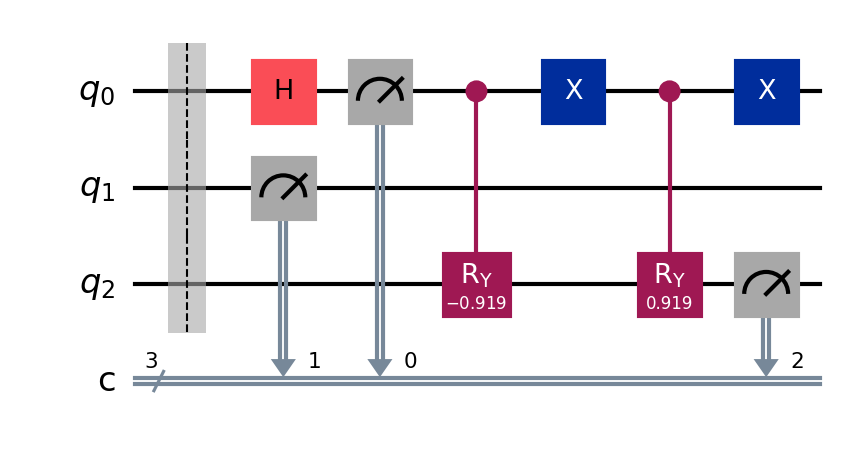
\includegraphics[width=0.95\columnwidth]{plots/qiskit/qcs/charge_qc.png}
    \caption{Quantum circuit used to extract Bob's charge expectation value in the charge teleportation protocol.}
    \label{fig:charge_qc}
\end{figure}

\subsection{Circuit Implementations and Simulation Strategy}

The teleportation protocols for both energy and charge observables were implemented as quantum circuits tailored to the specific measurement settings discussed throughout the thesis. 
Figure~\ref{fig:charge_qc} shows the charge-teleportation circuit \(Q_B\) measured at Bob’s site. The energy components \(H_B\) and \(V\) are shown in the appendix. The circuit closely follows the implementation used by Ikeda in the quantum energy teleportation experiment on superconducting hardware~\cite{Ikeda2023}.

Each circuit represents a specific measurement setting derived for a chosen value of \( J \) and \( h \), resulting in a corresponding optimal rotation angle \( \theta \) applied at Bob's site. The full derivation of these angles, and the basis in which Alice measures, are described in detail in Appendix~\ref{appendix:charge_teleportation}. These circuits are initialized to the entangled ground state of the relevant TFIM model by directly loading either the density matrix or the state itself into the circuit using a Qiskit initializer.

\subsubsection{Comparison with Ideal Numerical Simulations and Hardware Execution}

Unlike the ideal numerical simulations presented in earlier sections—which compute the exact expectation values from the full many-body ground state—the Qiskit-based approach simulates the entire teleportation protocol circuit including:
\begin{itemize}
    \item Preparation of the ground state as a density matrix (in simulation),
    \item Explicit measurements on Alice's qubit(s),
    \item Classical communication and conditional rotations,
    \item Measurement of Bob's observable.
\end{itemize}

The \textbf{simulated circuit execution} using Qiskit's `aer simulator` allows for a more realistic modeling of the teleportation process, but still assumes idealized, noise-free conditions. In contrast, results from \textbf{real quantum hardware} (discussed in Section~\ref{sec:hardware_results}) are subject to noise, decoherence, and gate errors, providing valuable insight into the feasibility of implementing QET-based protocols in practice.

This comparison between three levels of abstraction—analytical prediction, noiseless quantum circuit simulation, and real hardware execution—forms the foundation for assessing the practicality, robustness, and scalability of QET and charge teleportation protocols.

\subsection{Star-Coupled Hamiltonian Results}

\begin{figure*}
    \centering
    \subfloat[Energy, \( N = 1 \)]{
        
\includegraphics[width=0.3\textwidth]{plots/qiskit/Alice/N1_energy_vs_J.png}
    }
    \hfill
    \subfloat[Energy, \( N = 2 \)]{
        
\includegraphics[width=0.3\textwidth]{plots/qiskit/Alice/N2_energy_vs_J.png}
    }
    \hfill
    \subfloat[Energy, \( N = 3 \)]{
        
\includegraphics[width=0.3\textwidth]{plots/qiskit/Alice/N3_energy_vs_J.png}
    }

    \vspace{0.5em}

    \subfloat[Charge, \( N = 1 \)]{
        
\includegraphics[width=0.3\textwidth]{plots/qiskit/Alice/N1_charge_vs_J.png}
    }
    \hfill
    \subfloat[Charge, \( N = 2 \)]{
        
\includegraphics[width=0.3\textwidth]{plots/qiskit/Alice/N2_charge_vs_J.png}
    }
    \hfill
    \subfloat[Charge, \( N = 3 \)]{
        
\includegraphics[width=0.3\textwidth]{plots/qiskit/Alice/N3_charge_vs_J.png}
    }

    \caption{Qiskit simulation results for Energy (top) and Charge (bottom) teleportation protocol using the Star-Coupled Hamiltonian \( H^{(1)} \). All results are averaged over 10{,}000 shots.}
    \label{fig:qiskit_star_results}
\end{figure*}

We begin by examining the teleportation protocol under the star-type interaction Hamiltonian \( H^{(1)} \), where Alice interacts simultaneously with all other sites. Qiskit simulations were executed for both energy and charge teleportation protocols at system sizes \( N = 1, 2, 3 \), using the circuits introduced in the previous subsection. All simulations were averaged over 10{,}000 shots to approximate expectation values from discrete measurement outcomes.

Figure~\ref{fig:qiskit_star_results} presents the results of these simulations: the top row shows Bob’s extracted energy values, and the bottom row shows the corresponding charge values, all plotted against the coupling strength \( J \).

The data points in the figure represent the expectation values of the target observables, calculated by averaging over a large number of experimental runs, or "shots" ($n_{\text{shots}}$). The error bars correspond to the statistical uncertainty of this average, quantified by the standard error of the mean (SEM). The SEM is derived from the standard deviation of a single measurement and the total number of shots. A complete derivation of the statistical framework and the specific formulas used to calculate the SEM for both charge and energy observables is provided in Appendix~\ref{appendix:stats-analysis}.

\subsubsection*{Analysis and Comparison with Numerical Results}

As system size \( N \) increases, the \textbf{statistical noise} in the energy teleportation results becomes more pronounced. This effect is especially visible in panel (c), where the observable fluctuations for \( N = 3 \) exhibit substantial variance due to the low signal-to-noise ratio of energy teleportation at larger \( N \). Charge teleportation, in contrast, remains smooth and symmetric across all system sizes (Fig.~\ref{fig:qiskit_star_results}, bottom row), highlighting its superior robustness. This stands in clear opposition to the energy results, which show significant statistical fluctuations (Fig.~\ref{fig:qiskit_star_results}, top row).

Despite the increased variance, the Qiskit results align well with the ideal numerical simulations discussed in Section~\ref{sec:alice_hamiltonian}, both in structure and value range. Key features preserved include:
\begin{itemize}
    \item The \textbf{asymmetry} of energy teleportation with respect to Alice’s measurement result (bit \( b \)),
    \item The \textbf{mirror symmetry} in charge teleportation, where the two branches (for \( b = 0 \) and \( b = 1 \)) are nearly perfect reflections,
    \item The locations of the \textbf{maximal extracted values} near intermediate \( J \) values (around \( J \sim 1 \)).
\end{itemize}

In summary, these results demonstrate that Qiskit simulations capture the essential physics of the QET protocol under the Star-Coupled Hamiltonian. While averaging over many shots mitigates sampling noise, the energy protocol remains more sensitive to shot noise, especially at larger system sizes, whereas the charge protocol proves more reliable and scalable in this regime.

\subsection{Nearest Neighbors Hamiltonian Results}

\begin{figure*}[t!]
    \centering
    \subfloat[Energy, \( N = 2 \), \( \sigma_A = X_0 \)]{
        
\includegraphics[width=0.225\textwidth]{plots/qiskit/NearestNeighbors/X/N2_energy_vs_J.png}
    }
    \hfill
    \subfloat[Energy, \( N = 3 \), \( \sigma_A = X_0 \)]{
        
\includegraphics[width=0.225\textwidth]{plots/qiskit/NearestNeighbors/X/N3_energy_vs_J.png}
    }
    \hfill
    \subfloat[Energy, \( N = 2 \), \( \sigma_A = Y_0 \)]{
        
\includegraphics[width=0.225\textwidth]{plots/qiskit/NearestNeighbors/Y/N2_energy_vs_J.png}
    }
    \hfill
    \subfloat[Energy, \( N = 3 \), \( \sigma_A = Y_0 \)]{
        
\includegraphics[width=0.225\textwidth]{plots/qiskit/NearestNeighbors/Y/N3_energy_vs_J.png}
    }

    \vspace{0.5em}

    \subfloat[Charge, \( N = 2 \), \( \sigma_A = X_0 \)]{
        
\includegraphics[width=0.225\textwidth]{plots/qiskit/NearestNeighbors/X/N2_charge_vs_J.png}
    }
    \hfill
    \subfloat[Charge, \( N = 3 \), \( \sigma_A = X_0 \)]{
        
\includegraphics[width=0.225\textwidth]{plots/qiskit/NearestNeighbors/X/N3_charge_vs_J.png}
    }
    \hfill
    \subfloat[Charge, \( N = 2 \), \( \sigma_A = Y_0 \)]{
        
\includegraphics[width=0.225\textwidth]{plots/qiskit/NearestNeighbors/Y/N2_charge_vs_J.png}
    }
    \hfill
    \subfloat[Charge, \( N = 3 \), \( \sigma_A = Y_0 \)]{
        
\includegraphics[width=0.225\textwidth]{plots/qiskit/NearestNeighbors/Y/N3_charge_vs_J.png}
    }
    
    \caption{Qiskit simulation results for Energy (top) and Charge (bottom) teleportation using the nearest-neighbor Hamiltonian for both Alice's bases choices.}
    \label{fig:qiskit_nn}
\end{figure*}

We now analyze the behavior of the teleportation protocol under the nearest-neighbors Hamiltonian \( H^{(2)} \), where Alice interacts only with her immediate neighbor. As described in Section~\ref{sec:hamiltonians}, this modifies the communication channel between Alice and Bob from a direct interaction to one mediated by intermediate qubits. As in the previous case, we perform Qiskit simulations for both energy and charge teleportation, but now for system sizes \( N = 2 \) and \( N = 3 \) (since \( N = 1 \) reduces to the star interaction case). We consider two different measurement bases for Alice: \( \sigma_A = X_0 \) and \( \sigma_A = Y_0 \).

All simulations are averaged over a large number of shots to mitigate statistical noise: for \( N = 2 \), we average over 500{,}000 shots; for \( N = 3 \), we use 5{,}000{,}000 shots for the \( \sigma_A = X_0 \) basis and 500{,}000 for \( \sigma_A = Y_0 \). This aggressive sampling strategy is necessary due to the increasing weakness of the signal as the system grows in size and complexity.

\subsubsection*{Discussion}

The results shown in Figure~\ref{fig:qiskit_nn} present a significantly noisier behavior compared to the Star-Coupled Hamiltonian case. This increased noisiness arises from multiple sources:

\begin{itemize}
    \item \textbf{Propagation through intermediate sites:} In the nearest-neighbors model, Alice and Bob are no longer directly coupled. The teleportation signal must propagate through a chain of intermediate qubits, weakening the effect as \( N \) increases.
    \item \textbf{Statistical sampling noise:} The extracted signal, particularly for energy, is significantly smaller in magnitude. As a result, many more shots are required to resolve expectation values. This is clearly seen in the \( N = 3 \) case, where energy plots fluctuate heavily even after 5{,}000{,}000 shots.
    \item \textbf{Circuit separation:} Since the two components of Bob's energy — \( H^{(1)} \) and \( V \) — do not commute, they must be measured in separate circuits. This lack of coherence between components introduces additional statistical noise in the energy reconstruction.
\end{itemize}

It is also noteworthy that the \textbf{charge teleportation protocol is less sensitive} to these complications. Across both bases, the extracted charge shows a more stable and consistent pattern with respect to the coupling strength \( J \). Although the Y-basis appears to be a bit more sensitive to noise, which may result also from the small absolute values extracted by Bob. This emphasizes the importance of careful basis selection in realistic implementations.

These results underscore the relative robustness of charge-based teleportation in hardware-limited scenarios, as well as the practical challenges in implementing QET for energy observables in extended systems.

The increased statistical variance observed in the energy protocols is a direct consequence of error propagation: since the energy operator terms do not commute, they must be measured in separate circuit executions, summing their variances (see Appendix~\ref{appendix:stats-analysis} for derivation).

\subsection{Qiskit Experiment on Real Quantum Hardware}
\label{sec:hardware_results}

\begin{figure*}[t!]
    \centering
    \subfloat[Charge teleportation]{
        
\includegraphics[width=0.45\textwidth]{plots/qiskit/real_hw/real_hw_charge_vs_J.png}
        \label{subfloat:real_hw_charge_results}
    }
    \hfill
    \subfloat[Energy teleportation]{
        
\includegraphics[width=0.45\textwidth]{plots/qiskit/real_hw/real_hw_energy_vs_J.png}
        \label{subfloat:real_hw_energy_results}
    }
    \caption{Experimental protocol results obtained from real quantum hardware for \( N = 1 \), using Alice’s \( \sigma_A = X_0 \) basis. Each point represents an independent execution for a fixed value of coupling \( J \).}
    \label{fig:real_hw_results}
\end{figure*}

To complete the analysis, we implement the teleportation protocol on an actual quantum processor, the \texttt{ibm\_torino} QPU, via the \texttt{IBM Quantum Platform}. The experiment was conducted for the minimal configuration with \( N = 1 \) using Alice's basis \( \sigma_A = X_0 \), which corresponds to both the \( H^{(1)} \) and \( H^{(2)} \) models in this simple setting. The charge and energy observables were measured separately using the circuits introduced earlier.

The results, shown in Figure~\ref{fig:real_hw_results}, provide crucial insight into the protocol's performance in the presence of realistic device noise. A key observation is a significant positive offset in the measured expectation values compared to the ideal simulations. This is particularly evident at \( J=0 \), where both the charge and energy signals are positive, regardless of Alice's classical bit choice (\( a=0 \) or \( a=1 \)). Such a systematic shift could be caused by various factors, including an imperfectly prepared ground state, decoherence, or measurement readout errors.

For the energy teleportation protocol, this offset proves to be critical. As seen in Figure~\ref{subfloat:real_hw_energy_results}, the expectation values for the \( a=0 \) branch remain positive across the entire range of \( J \). Since the protocol's security relies on encoding key bits in the sign of the measured observable, the persistent positive sign means the protocol fails to produce a distinguishable key. Without sophisticated error correction to compensate for this offset, energy teleportation is not viable in this noisy environment.

The charge teleportation protocol demonstrates its enhanced robustness. While it is also affected by the initial offset at \( J=0 \), the signal strength for the \( a=0 \) branch grows sufficiently negative as \( J \) increases. As shown in Figure~\ref{subfloat:real_hw_charge_results}, the signal overcomes the systematic positive bias, re-establishing the clear sign separation between the \( a=0 \) and \( a=1 \) branches. This confirms that for a large enough coupling \( J \), the charge protocol remains functional and can reliably encode key bits.

This experiment provides practical validation that observable teleportation is feasible on near-term quantum hardware using only LOCC. More importantly, it highlights that while the underlying mechanism works, the choice of observable is paramount. The pronounced resilience of charge teleportation against systematic hardware noise reinforces our central claim that it is a more practical and robust candidate for QKD applications.
